\documentclass[modern]{aastex62}

% Load the corTeX style definitions
% All the packages
\usepackage{url}
\usepackage{amsmath}
\usepackage{mathtools}
\usepackage{amssymb}
\usepackage{natbib}
\usepackage{graphicx}
\usepackage{calc}
\usepackage{etoolbox}
\usepackage{xspace}
\usepackage[T1]{fontenc} % https://tex.stackexchange.com/a/166791
\usepackage{textcomp}
\usepackage{ifxetex}
\ifxetex
\usepackage{fontspec}
\defaultfontfeatures{Extension = .otf}
\fi
\usepackage{fontawesome}
\usepackage{listings}

% Shorthand for this paper
\newcommand{\Python}{\textsf{Python}\xspace}
\newcommand{\cpp}{\textsf{C}++\xspace}
\newcommand{\starry}{\textsf{starry}\xspace}
\newcommand{\spiceypy}{\textsf{spiceypy}\xspace}
\newcommand{\tf}{\textsf{TensorFlow}\xspace}
\newcommand{\tess}{\emph{TESS}\xspace}

% References to text content
\newcommand{\documentname}{\textsl{article}}
\newcommand{\figureref}[1]{\ref{fig:#1}}
\newcommand{\Figure}[1]{Figure~\figureref{#1}}
\newcommand{\figurelabel}[1]{\label{fig:#1}}
\renewcommand{\eqref}[1]{\ref{eq:#1}}
\newcommand{\Eq}[1]{Equation~(\eqref{#1})}
\newcommand{\eq}[1]{\Eq{#1}}
\newcommand{\eqalt}[1]{Equation~\eqref{#1}}

% Add code, proof, and animation hyperlinks
\definecolor{linkcolor}{rgb}{0.1216,0.4667,0.7059}
\newcommand{\codeicon}{{\color{linkcolor}\faFileCodeO}}
\newcommand{\prooficon}{{\color{linkcolor}\faPencilSquareO}}
\newcommand{\codelink}[1]{\href{https://github.com/rodluger/earthshine/blob/3b1b4e288b46cb8823ff70e269c2acbf3303b236/notebooks/#1.ipynb}{\codeicon}\,\,}


% Define a proof environment for open source equation proofs
\newtagform{eqtag}[]{(}{)}
\newcommand{\currentlabel}{None}
\newenvironment{proof}[1]{%
\ifstrempty{#1}{%
\renewtagform{eqtag}[]{\raisebox{-0.1em}{{\color{red}\faPencilSquareO}}\,(}{)}%
}{%
\renewtagform{eqtag}[]{\prooflink{#1}\,(}{)}%
}%
\usetagform{eqtag}%
\renewcommand{\currentlabel}{#1}
\align%
}{%
\endalign%
\renewtagform{eqtag}[]{(}{)}%
\usetagform{eqtag}%
\message{<<<\currentlabel: \theequation>>>}%
}

% Define the `oscaption` command for open source figure captions
\newcommand{\oscaption}[2]{\caption{#2 \codelink{#1}}}

% Code examples
\definecolor{codegreen}{rgb}{0,0.6,0}
\definecolor{codegray}{rgb}{0.5,0.5,0.5}
\definecolor{codepurple}{rgb}{0.58,0,0.82}
\definecolor{backcolour}{rgb}{0.95,0.95,0.95}
\lstdefinestyle{mystyle}{
    backgroundcolor=\color{backcolour},
    commentstyle=\color{codegreen},
    keywordstyle=\color{magenta},
    numberstyle=\tiny\color{codegray},
    stringstyle=\color{codepurple},
    basicstyle=\small\ttfamily,
    breakatwhitespace=false,
    breaklines=true,
    captionpos=b,
    keepspaces=true,
    numbers=left,
    numbersep=5pt,
    showspaces=false,
    showstringspaces=false,
    showtabs=false,
    tabsize=2,
    aboveskip=1em,
    belowskip=1em,
    keywords=[2]{map},
    keywordstyle=[2]{\color{black!80!black}},
    upquote=true
}
\lstset{style=mystyle}

% Typography obsessions
\setlength{\parindent}{3.0ex}
\renewcommand\quad{\hskip\fontdimen3\font}


\usepackage{xcolor}
\usepackage{xspace}
\newcommand{\TESS}{\emph{TESS}\xspace}
\newcommand{\todo}[1]{\textcolor{red}{#1}}

% Bibliography stuff
\bibliographystyle{aasjournal}

% Begin!
\begin{document}

% Title
\title{\TESS Photometric Mapping of a Terrestrial Planet in the Habitable Zone: 
       Detection of Clouds, Oceans, and Continents}
%\title{Detection of Continents on a Habitable-Zone Terrestrial Planet with \TESS}

% Author list
\author[0000-0002-0296-3826]{Rodrigo Luger}
\email{rluger@flatironinstitute.org}
\affil{Center~for~Computational~Astrophysics, Flatiron~Institute, New~York, NY}
%
\author[0000-0002-9328-5652]{Megan Bedell}
\affil{Center~for~Computational~Astrophysics, Flatiron~Institute, New~York, NY}
%
\author{Roland K. Vanderspek}
\affil{Kavli Institute for Astrophysics and Space Research, Massachusetts 
       Institute of Technology, Cambridge, MA}
%
\author{Christopher J. Burke}
\affil{Kavli Institute for Astrophysics and Space Research, Massachusetts 
       Institute of Technology, Cambridge, MA}

\begin{abstract}
\todo{[maybe change first sentences to focus on planet mapping \& give the game 
away less?]} The Transiting Exoplanet Survey Satellite (\TESS) mission is a 
targeted effort to detect planets smaller than Neptune around bright, nearby stars. 
While \TESS is already enjoying great success with the discovery of many new worlds, 
the strongest signal in its data is typically ignored, as it lurks in the background 
of every camera pixel. In this work, we extract this signal and demonstrate that 
it is consistent with a terrestrial planet with a rotation period of 1 day. 
Using a spherical harmonic-based reflection model developed as an extension of 
the \starry package, we are able to reconstruct the surface features of this rocky 
world. We recover a time-variable albedo map of the planet including persistent 
regions which we interpret as continental features and cloud banks. 
We argue that this planet represents the most promising detection of a habitable 
world to date, although the potential intelligence of any life on it is yet to 
be determined.
\end{abstract}

\keywords{methods: data analysis, techniques: photometric, planets and satellites: 
          oceans, planets and satellites: surfaces, planets and satellites: 
          terrestrial planets}

% Introduction
\section{Introduction}
\label{sec:intro}

%Resolving the features of planetary atmospheres and surfaces with precise 
%photometry is a crucial 
Precise photometry obtained over long periods of time can reveal the atmospheric 
and surface features of an exoplanet through the method known as phase mapping. 
\todo{(literature background \& citations)}

A new source of precise photometry is the Transiting Exoplanet Survey Satellite 
\citep[\TESS; ][]{Ricker2015}. 
Launched in April 2018, \TESS has... \todo{(summary of \TESS's capabilities, 
citations to planet discoveries etc)}

One intriguing feature of the \TESS photometric data products is a highly 
time-variable signal represented in the diffuse background across virtually 
all camera pixels. 
\todo{(talk abt Earthshine without naming it)} 
The signal has been widely attributed to a planet which we will call Sol d.

Previous attempts to map this planet from the exoplanet community have suggested 
the presence of localized surface features, but their resolving power has been 
severely limited by the duration of observations \citep{Cowan2009}. 
\TESS offers precise 2-minute cadence data spanning a wide range of illumination 
phases, enabling a level of spatial and temporal resolving power that is 
unprecedented in the exoplanetary phase mapping literature. 

Moreover, recent advances in fast analytic computation of spherical harmonics 
have made the reconstruction of such detailed maps more feasible than ever. 
\todo{(STARRY)}

In this work, we build on this methodological foundation to perform 
reflected-light mapping of planetary surface features on Sol d. 
We give an overview of the \TESS data used in Section \ref{sec:data}. 
In Section \ref{sec:methods}, we describe the methods employed to infer a map 
from these data, including the adaptation of the \starry algorithm to reflection 
mapping, the modeling of spacecraft-related systematics, and the likelihood and 
priors used. 
We present results in Section \ref{sec:results} and make comparison of these 
findings to state-of-the-art terrestrial planet maps from the literature in 
Section \ref{sec:discussion}. 
Finally, we conclude in Section \ref{sec:conclusion} with a look at future 
prospects for phase-curve mapping of terrestrial exoplanets.

\section{Data}
\label{sec:data}

\todo{(background extraction from 2-minute cadence targets)}

\todo{TJD = BJD - 2457000}

\todo{75 light curves in S1, 20 in S2}
\todo{912,605 data points in total}

\todo{(outlier rejection method, trim down to x number of high-SNR lightcurves 
for computational tractability)}

We subtract the estimated background from each signal.

Figure showing lightcurves for various targets: Figure~\ref{fig:data}.

\begin{figure}[ht!]
    \begin{centering}
    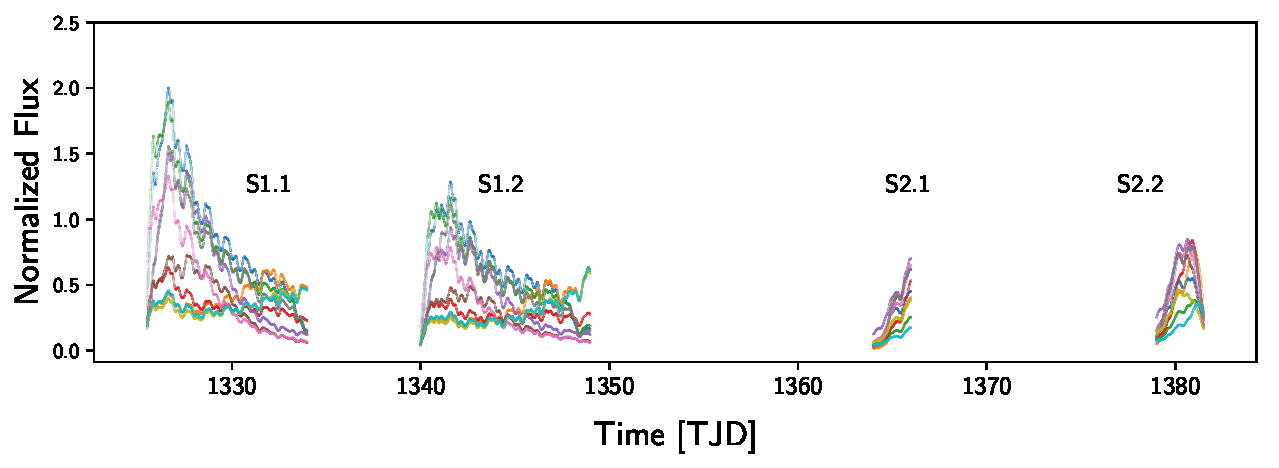
\includegraphics[width=\linewidth]{figures/data.pdf}
    \caption{\label{fig:data}
             Normalized background flux in each of ten postage stamps
             for each of Sectors 1 and 2. Cadences where Sol d was
             below or very close to the edge of the sunshade were masked.
             While the planet is in view for the majority of both orbits
             in Sector 1, it is only visible in the data at the very end
             of each orbit in Sector 2.
             \codelink{earthshine_S1_S2}
             }
    \end{centering}
\end{figure}

\section{Methods}
\label{sec:methods}

\subsection{Orbital Modeling}
\label{sec:orbit}

We downloaded 
\footnote{\url{https://archive.stsci.edu/missions/tess/models/}}
the Solar System and \tess ephemeris data for
Sectors 1 and 2 and used \spiceypy \citep{Acton1996, Acton2017, Annex2017}
to convert the TJD timestamps to 
ephemeris time (ET). We then used the \textsf{spkezr} utility to compute
the relative positions of Sol, Sol d, and \tess for every cadence
in our dataset in the J2000 equatorial reference frame. In this right-handed
coordinate frame, Sol d is centered at the origin, the $y$ axis points along the 
planet's spin axis, and the $x$ axis points toward the vernal equinox. We
do not apply any light travel correction, as the expected delay is on the order
of a few seconds.

At any given cadence, we rotate Sol d about its spin axis to the correct phase,
assuming a rotational period of $1.00$ day. We determine the initial rotation
phase of Sol d by computing the Sol d Rotation Angle (ERA), given by \citep{Urban2013}
%
\begin{align}
\mathrm{ERA} = 360^\circ(0.7790572732640 + 1.00273781191135448 \, t_U) \, \mathrm{mod} \, 360^\circ
\end{align}
%
where $t_U = t - 2451545.0$. At $t = t_0 = 2458325.5$, the first timestamp in our dataset,
we find $\mathrm{ERA} = 303.4^\circ$, meaning the vernal equinox will be aligned with
the prime meridian $360^\circ - 303.4^\circ = 56.6^\circ = 3.77$ hours past $t_0$.
%
Finally, we rotate the frame to align
\tess with the $+z$ axis, with the spin vector of Sol d along the $y-z$ plane.

\begin{figure}[ht!]
    \begin{centering}
    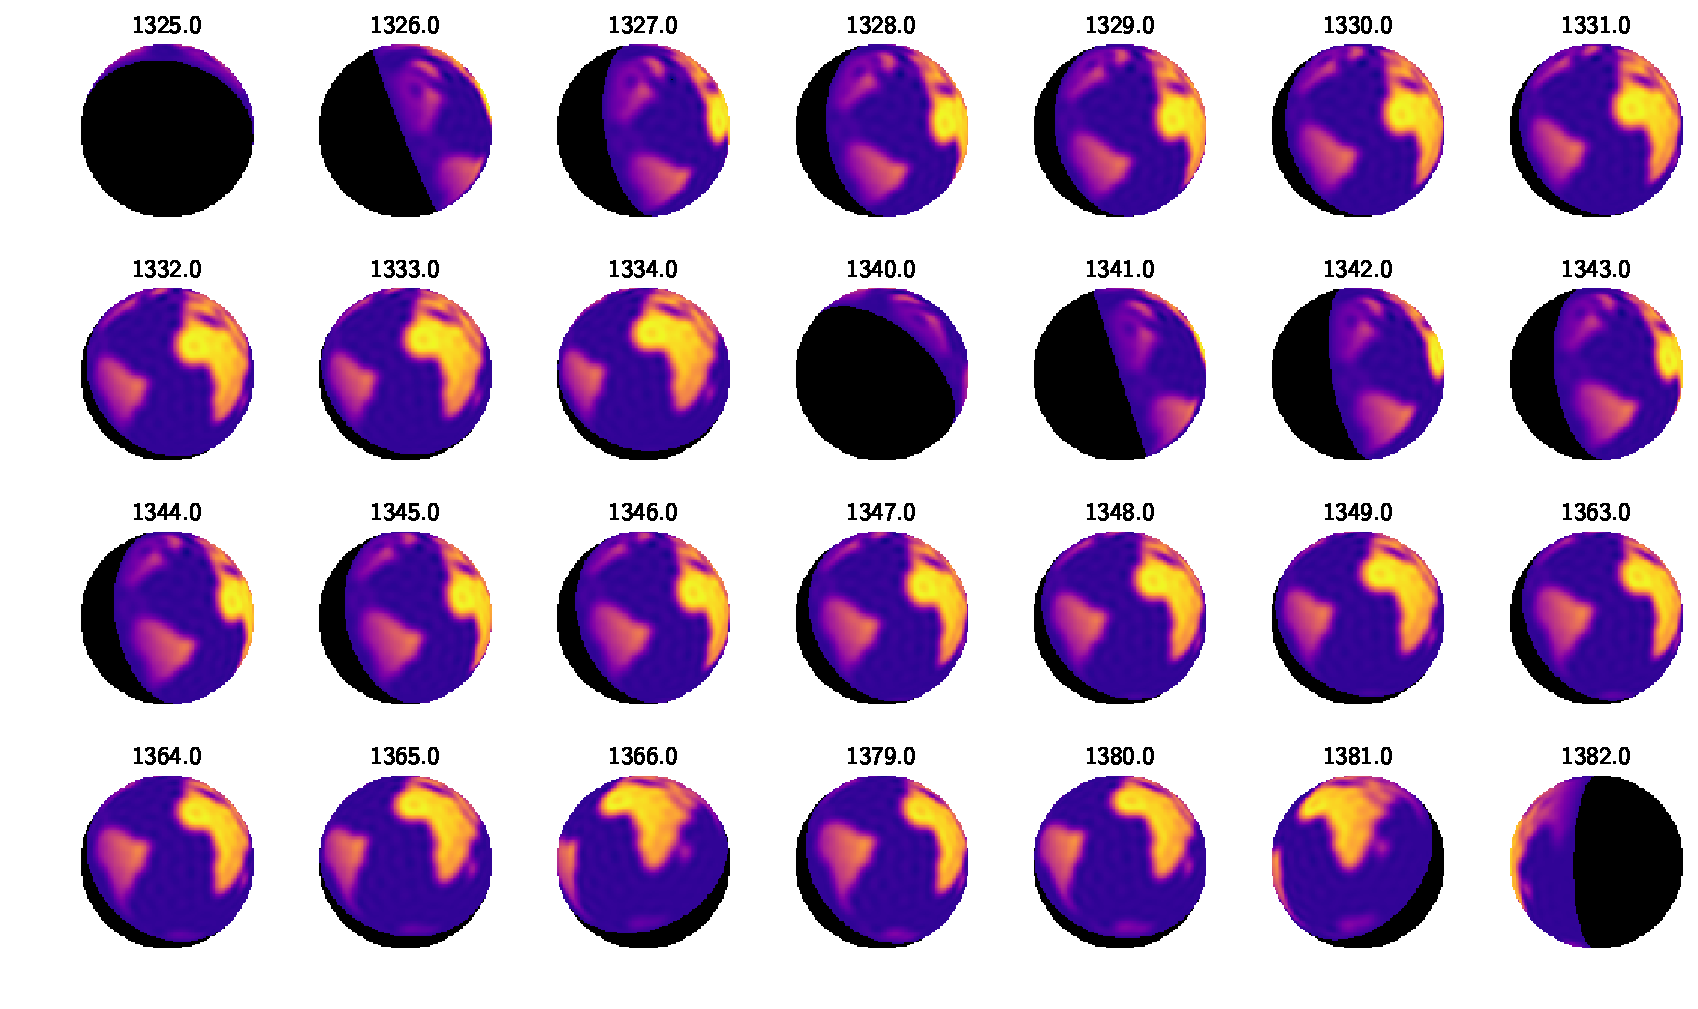
\includegraphics[width=\linewidth]{figures/phases.pdf}
    \caption{\label{fig:phases}
             \tess view of Sol d on every date in Sectors 1
             and 2 that was included in the regression. Each image is
             labeled with the corresponding timestamp in TJD. The images
             shown here correspond to current models of the continental coverage
             of Sol d, not to the map inferred in this study.
             \codelink{EarthView}
             }
    \end{centering}
\end{figure}

Figure~\ref{fig:phases} shows the view \tess has of Sol d on each of the dates
in our dataset; these images were produced by applying the sequences of rotations
described above. The planet is illuminated by Sol assuming it is a point source,
and the night side is shaded black. The map of Sol d shown in this figure is 
based on current models of the actual distribution of continents on the planet.
Note that although the images are computed an integer number of rotation periods
apart, the planet appears to slowly rotate over the course of the observation.
This is because of the orbit of \tess, which changes its vantage point relative
to Sol d over the course of its 13 day orbit.

\subsection{Systematics Modeling}
\label{sec:systematics}

While the astrophysical signal that we wish to analyze is present in all 
extracted lightcurves, its strength is modulated by time-variable systematics 
that are correlated but not identical across all postage stamps, since the
illumination of the CCD by Sol d is strongly inhomogeneous. A physical
model of the reflections and scattering that gives rise to the
signal of Sol d on the \tess detector is beyond the scope of this work. Instead,
we treat this as a de-trending problem, where the signal we wish to fit is
shared by all postage stamps, but multiplied by a systematic signal that is
different for each target. This problem is precisely what the technique of
pixel-level decorelation \citep[PLD;][]{Deming2015, Luger2016, Luger2018a}
seeks to address. In PLD, one computes the sum over all light curves at each
point in time, and uses this quantity to normalize each of the individual
light curves. Since (by assumption) each light curve is the product of the astrophysical
signal and the systematics signal, this procedure divides out the astrophysical
signal, producing a basis of vectors that contain \emph{only} functions of the
systematics. This now serves as a ``clean'' basis one can then use to fit the
data, with minimal risk of fitting out astrophysical signals.

We therefore construct a design matrix $\mathbf{B}$ out of the PLD basis. To
increase the flexibility of the systematics model, we append to $\mathbf{B}$ 5 orthogonal
polynomials in time for each of the two orbits of \tess in each sector.
The systematics model $\mathbf{p}$ for the $n^\mathrm{th}$ signal is thus
%
\begin{align}
\mathbf{p}_n = \mathbf{B} \mathbf{w}_n
\end{align}
%
where $\mathbf{w}_n$ are the weights of each regressor.
Since we solve for different weights for each of the 75 light curves in Sector 1
and 20 light curves in Sector 2, our systematics model has
$75 \times (75 + 2 \times 5) + 20 \times (20 + 2 \times 5) = 6,975$ free parameters.
The total number of data points is $912,605$, so overfitting is not particularly
concerning; nevertheless, we impose an L2 prior on the weights with
standard deviation $\sigma_B = 0.1$ (see \S\ref{sec:model}).

\subsection{Reflected-Light Mapping with \starry}
\label{sec:starry}

We model the astrophysical component of the signal---the rotational modulation
of Sol d in reflected light---using the \starry code package \citep{Luger2019}.
\starry computes phase curves and occultation light curves for bodies whose
surfaces are expressed as a sum of spherical harmonics. 
The algorithm works by first transforming
from spherical harmonic coefficients to coefficients in the polynomial basis $\tilde{p}$, whose
terms are of the form $x^i y^j z^k$ for (non-negative) integer $i$ and $j$ 
and $k = 0$ or $1$. \citet{Luger2019} showed how to compute the visible
flux by integrating each of the terms in $\tilde{p}$ across the visible
surface of the projected disk. For unocculted spheres observed in emitted
light, the area of integration is the full disk, which makes the integration
trivial: the flux contribution from each term in $\tilde{p}$ is a constant
easily computed via recursion relations involving factorials. The algorithm is
thus extremely fast and very precise.

However, in the present work, we are interested in \emph{reflected} light, so we must
account for the illumination by the star, which varies smoothly
across the dayside of the planet but whose derivative discontinuously changes at the 
terminator, beyond which the illumination is zero everywhere. This requires
two modifications to the \starry algorithm: we must (1) weight all integrands
by the illumination function on the dayside, and (2) modify the integration
limits to truncate the integrals at the day/night terminator.

\begin{figure}[ht!]
    \begin{centering}
    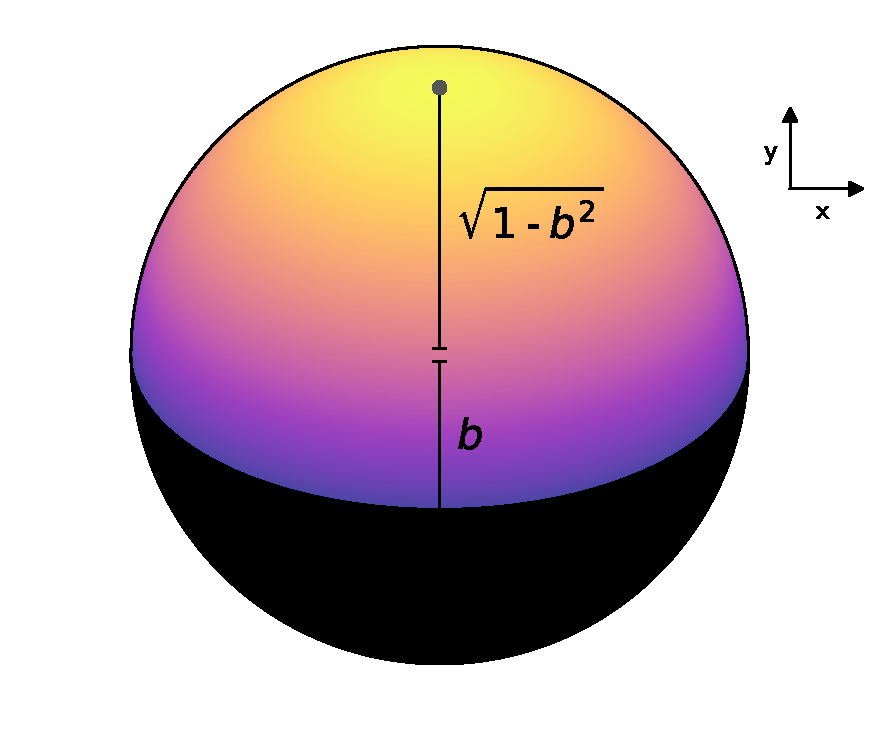
\includegraphics[width=0.4\linewidth]{figures/geometry.pdf}
    \caption{\label{fig:geometry}
             Geometry of the \starry model in reflected light. In this frame, 
             the $y$ axis points up, 
             the $x$ axis points to the right, and the $z$ axis points out of the page.
             The planet has unit radius and sits at the origin, while
             the illumination source is along the $y-z$ plane, with the sub-stellar point is
             marked by a dot. The semi-major axis of the terminator is unity, and
             the semi-minor axis of the terminator is denoted $b$. The night side
             is colored black.
             \codelink{Geometry}
             }
    \end{centering}
\end{figure}

Let us consider a right-handed coordinate frame in which the planet has unit 
radius and is located at the origin, the illumination source is along the $y-z$
plane, and the sub-stellar point is on the $+y$ axis at $x = 0$
(see Figure~\ref{fig:geometry}). In this frame, the terminator is a segment of
an ellipse, with semi-major axis $a=1$ aligned with the $x$ axis and
semi-minor axis $b$. It is straightforward to show that the sub-stellar point
is located at $y=\sqrt{1 - b^2}$ and the illumination is given by
%
\begin{align}
    I(b; x, y) &= 
    \begin{dcases}
        \sqrt{1 - b^2}y - bz & 
            \quad\quad\quad\quad\quad\quad\quad\quad\quad\quad 
            y \geq -b \sqrt{1 - x^2}
        \\
        0 & 
            \quad\quad\quad\quad\quad\quad\quad\quad\quad\quad 
            \mathrm{otherwise}
    \end{dcases}
    \quad ,
    \label{eq:illum}
\end{align}
%
where $z = \sqrt{1 - x^2 - y^2}$.
%
Since the illumination function is just a polynomial in $x$, $y$, and $z$,
weighting the terms in $\tilde{p}$ by this function keeps all terms within the
polynomial basis.
Provided we always rotate the problem such that the
sub-stellar point lies along the $+y$ axis as above, the limits of integration
are $-1 \leq x \leq 1$ and $b\sqrt{1 - x^2} \leq y \leq \sqrt{1 - x^2}$.
Computing the total reflected flux for any surface map is therefore a matter
of solving integrals of the form
%
\begin{align}
    J_{ijk}(b) &= \int_{-1}^{1} \int_{b\sqrt{1 - x^2}}^{\sqrt{1 - x^2}} x^i y^j z^k \mathrm{d} y \ \mathrm{d} x
    \nonumber\\
    &=
    \frac{
        \Gamma\left(\frac{i + 1}{2}\right) \Gamma\left(\frac{j + 1}{2}\right)
    }{
        2 \Gamma\left(\frac{i + j + k + 4}{2}\right)
    }
    \begin{dcases}
        0
        &
        \quad\quad\quad\quad\quad\quad\quad\quad\quad\quad 
        i \, \mathrm{odd}
        %
        \\
        %
            1 - b^{j + 1}
        & 
        \quad\quad\quad\quad\quad\quad\quad\quad\quad\quad 
        k = 0
        %
        \\
        %
        \frac{\sqrt{\pi}}{2} - b^{j + 1}\Gamma\left(\frac{j + 4}{2}\right)
        {_2\tilde{F}_1} \left( -\frac{1}{2}, \frac{j + 1}{2}; \frac{j + 3}{2}; b^2\right)
        & 
        \quad\quad\quad\quad\quad\quad\quad\quad\quad\quad 
        k = 1
    \end{dcases}
    \quad ,
    \label{eq:integral}
\end{align}
%
where ${_2\tilde{F}_1}$ is the regularized hypergeometric function. For all values
of $i$, $j$, and $k$ in $\tilde{p}$, ${_2\tilde{F}_1}$ reduces to simple
trigonometric functions involving $b$. Moreover, it is straightforward to
derive recursion relations for $J_{ijk}(b)$, making its evaluation extremely fast.
We implemented the algorithm for computing $J_{ijk}(b)$ in the development version
of \starry
\footnote{\url{https://github.com/rodluger/starry/tree/linear}}
and will be discussed in detail in upcoming work.

\begin{figure}[ht!]
    \begin{centering}
    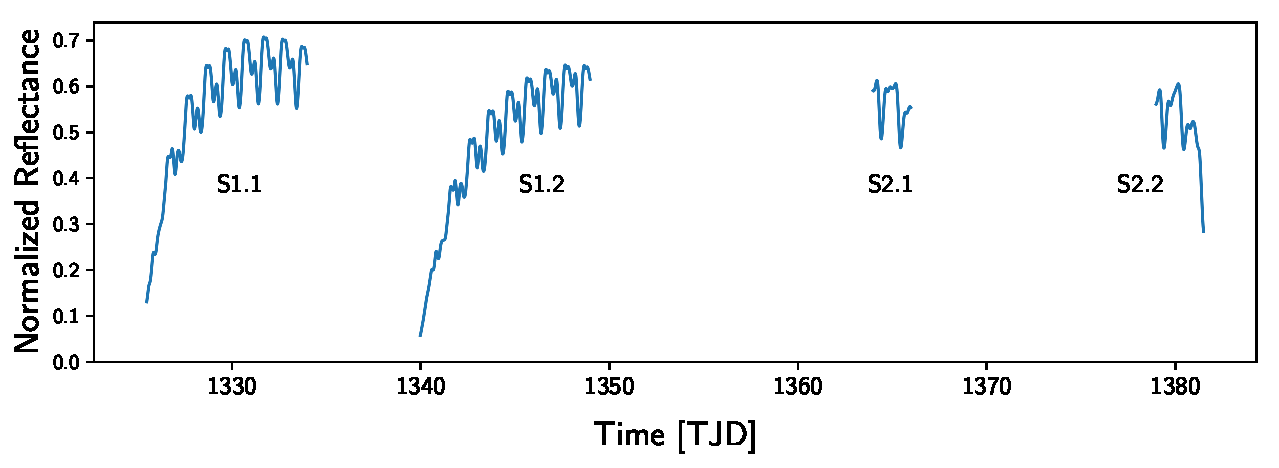
\includegraphics[width=\linewidth]{figures/starry_model.pdf}
    \caption{\label{fig:starry_model}
             Normalized surface reflectance versus time for the maximum
             likelihood \starry model in each of the four orbits of \tess
             in Sectors 1 and 2.
             \codelink{earthshine_S1_S2}
             }
    \end{centering}
\end{figure}

As with the systematics model (\S\ref{sec:systematics}), the model
for the astrophysical signal is \emph{linear}: the signal $\mathbf{s}$ 
is a linear operation on the vector of spherical harmonic coefficients 
that describes the body's surface:
%
\begin{align}
    \mathbf{s} = \mathbf{A} \mathbf{y}
\end{align}
%
where $\mathbf{A}$ is the design matrix and $\mathbf{y}$ is the vector of spherical harmonic coefficients. 
Note that in \cite{Luger2019}, $\mathbf{y}$ describes the emissivity of the surface,
but here we will use it to represent the \emph{albedo} of the planet.
We choose a maximum spherical harmonics degree $l_{max} = 15$ for our fits,
noting that increasing $l_{max}$ above this value does not significantly
improve the quality of our fits. At the equator, $l = 15$ corresponds to
a resolution on the order of $180^\circ/15 = 12^\circ$.

Finally, for reference, in Figure~\ref{fig:starry_model} we plot the
\starry model for our maximum likelihood fit (\S\ref{sec:results}). The
sharp rise at the beginning of each orbit in Sector 1 is due to the changing
vantage point of \tess as Sol d transitions from a thin crescent to full phase.

\subsection{Full Model and Likelihood Function}
\label{sec:model}

Our full model for each light curve is simply the product of the 
systematics model $\mathbf{p}_n$ (different for each target) and
the \starry model $\mathbf{s}$ (shared by all targets). Since we happen
to know the exact distance $\mathbf{r}$ between \tess and Sol d at all times
(\S\ref{sec:orbit}), we also include the inverse square of $\mathbf{r}$ 
as a multiplicative term. The model for the flux timeseries
in the $n^\mathrm{th}$ postage stamp is therefore
%
\begin{align}
    \label{eq:model}
    \mathbf{m}_n = (\mathbf{r}^{-2}) \circ (\mathbf{B} \mathbf{w}_n) \circ (\mathbf{A} \mathbf{y})
\end{align}
%
where $\circ$ denotes the element-wise product of two vectors.

We solve Equation~(\ref{eq:model}) for the weights $\mathbf{w}_n$ and $\mathbf{y}$
by maximizing the negative log likelihood function in two separate steps. In the
first step, we take advantage of the linearity of the problem to perform a fast,
semi-analytical optimization to obtain a starting guess for the weights. In the
second step, we apply additional constraints to prevent overfitting and ensure
an albedo in the range $[0, 1]$ everywhere on the surface.

In the first step, we initialize the \starry model to unity and iteratively
solve for $\mathbf{w}_n$ and $\mathbf{y}$ by solving the L2-regularized
least squares problem \citep[see, e.g., \S2.1 in][]{Luger2018a}.
We assume zero-mean Gaussian priors for the weights:
%
\begin{equation}
    \begin{aligned}
        \mathbf{w}_n \sim \mathcal{N}(0, \sigma_w^2)
    \end{aligned}
    \qquad\qquad\qquad\qquad
    \begin{aligned}
        \mathbf{y} \sim \mathcal{N}(0, \sigma_y(l)^2)
    \end{aligned}\, ,
\end{equation}
%
with $\sigma_w = 0.1$ and 
%
\begin{align}
    \sigma_y(l) &=
    \begin{dcases}
        1.75\times 10^{-5} \, l^\frac{3}{2} & 
            \quad\quad\quad\quad\quad\quad\quad\quad\quad\quad 
            l < 2
        \\
        1.40\times 10^{-4} \, l^{-\frac{3}{2}} & 
            \quad\quad\quad\quad\quad\quad\quad\quad\quad\quad 
            l \geq 2
    \end{dcases}
    \, ,
\end{align}
%
where $l$ is the spherical harmonic degree. The latter prior was chosen
by trial-and-error and was adjusted to keep the albedo positive
everywhere on the surface. Note, importantly, that we do
not fit for the coefficient of the constant $Y_{0,0}$ spherical harmonic,
but instead fix it to unity. Since the solutions obtained in this step are merely
used as a starting point for the second step (see below), the choice of prior 
at this stage has minimal impact on our results.

In general, we find that the iterative scheme converges within about 50 
iterations. However, since it is strongly regularized, the model significantly
underfits the data. In the second step, we remove our L2 prior on the spherical
harmonic coefficients and instead regularize the actual surface albedo, which
we compute on a uniform spherical grid with 50,000 points. We enforce a 
uniform prior in the range $[0, 1]$, with an exponential drop on either 
side. We additionally impose a constraint on the power spectrum of the
inferred map, \todo{bla bla}.


Our full negative log likelihood function in this step is therefore
%
\begin{align}
    -\log\mathcal{L} \, = \, 
        &\frac{1}{2}(\mathbf{f} - \mathbf{m})^\top \Sigma^{-1} (\mathbf{f} - \mathbf{m}) \, + \nonumber \\
        &\frac{1}{2}\mathbf{w}^\top \Lambda_w^{-1} \mathbf{w} \, + \nonumber \\
        &\frac{1}{2}(\mathbf{a_-} + 1 - \mathbf{a_+})^\top \Lambda_a^{-1} (\mathbf{a_-} + 1 - \mathbf{a_+}) \, + \nonumber \\
        &\frac{1}{2}(\rho - l^{-\gamma})^\top \Lambda_\rho^{-1} (\rho - l^{-\gamma}) \, + \nonumber \\
        &\frac{1}{2} \frac{\gamma^2}{\sigma_\gamma^2}
        \quad,
\end{align}
%
where \todo{explain all this stuff.}

All of these constraint break the linearity of the problem, so we must
now use a non-linear optimizer. We use the 
\textsf{AdamOptimizer} method in the \tf package \citep{Abadi2015}
to maximize the negative log likelihood.




\todo{(details of TensorFlow optimization)}

\section{Results}
\label{sec:results}

\begin{figure}[t!]
    \begin{centering}
    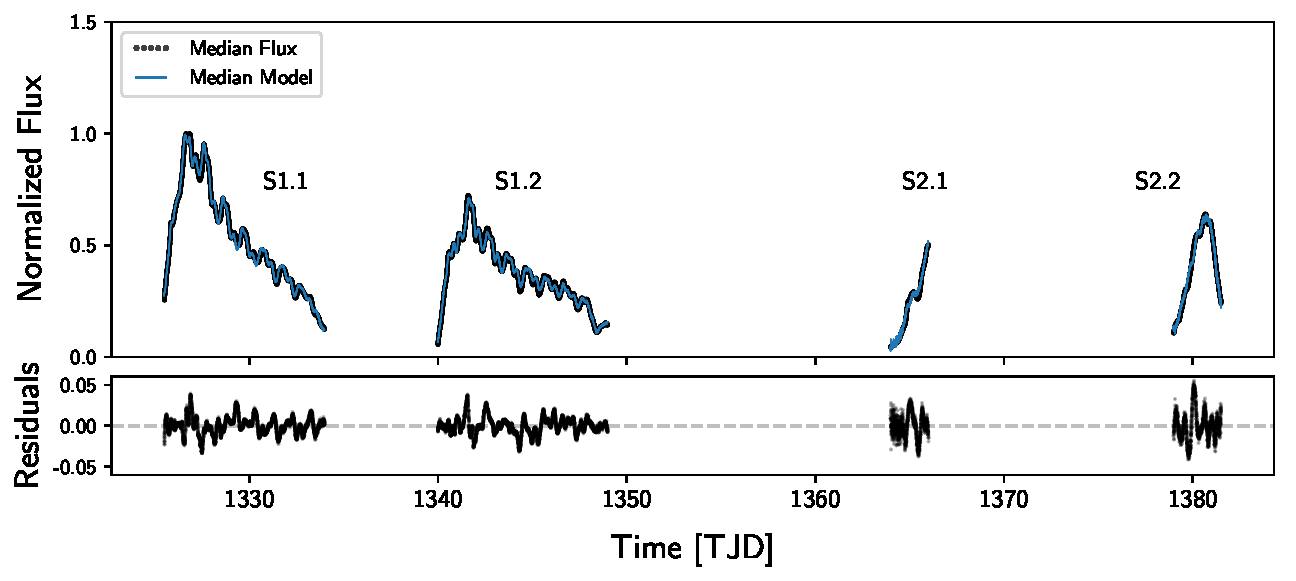
\includegraphics[width=\linewidth]{figures/model.pdf}
    \caption{\label{fig:model}
             \emph{Top:} Median flux across all postage stamps (black) and
             the median maximum likelihood model (blue) across Sectors 1 and 2.
             \emph{Bottom:} Median residuals about the maximum likelihood fit.
             \codelink{earthshine_S1_S2}
             }
    \end{centering}
\end{figure}

\begin{figure}[t!]
    \begin{centering}
    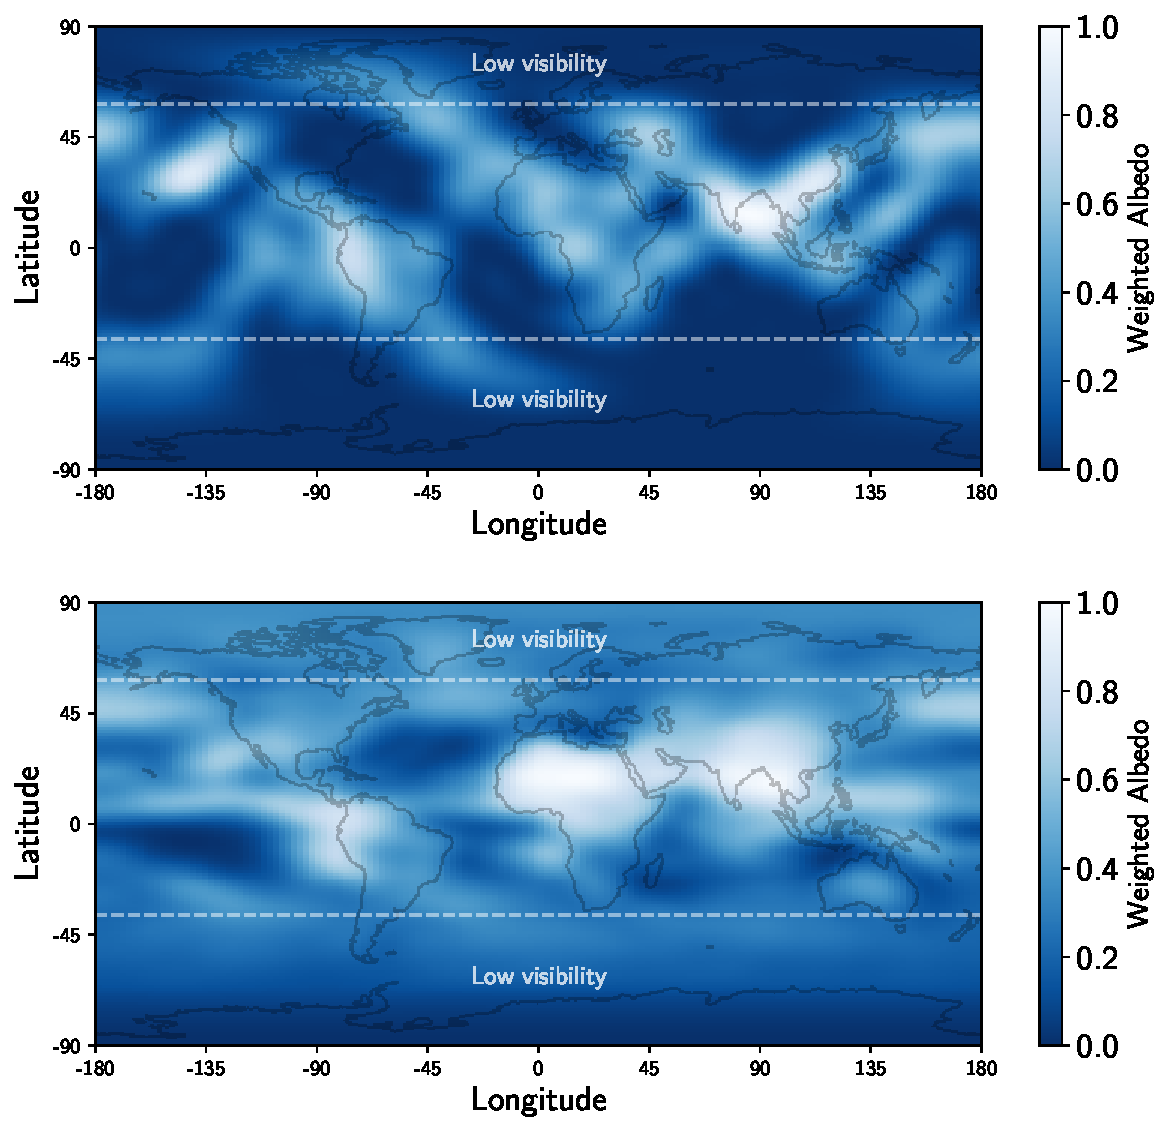
\includegraphics[width=\linewidth]{figures/map.pdf}
    \caption{\label{fig:map}
             \emph{Top:} The maximum likelihood model for the surface albedo
             of Sol d, weighted by the visibility across Sectors 1 and 2. The
             dashed white lines indicate latitudes above/below which the
             visibility drops below 50\%. Black contours indicate coastlines
             derived from current state-of-the-art models of the surface geography 
             of Sol d.
             \emph{Bottom:} Actual corrected surface reflectance in the red band of the
             \emph{VIIRS} imager, averaged over the same date range, band limited
             to $l_\mathrm{max} = 15$, and weighted
             by the same visibility function. This bandpass covers only about one
             quarter of the \tess bandpass, so deviations between the two images
             are to be expected.
             \codelink{earthshine_S1_S2}
             }
    \end{centering}
\end{figure}

Figure~\ref{fig:model} shows the median model.  \todo{More on this here.}

The top panel of Figure~\ref{fig:map} shows the maximum likelihood map of Sol d.
\todo{More on this here.}

The bottom panel of Figure~\ref{fig:map} shows the corrected surface
reflectance obtained from the
Visible Infrared Imaging Radiometer Suite (\emph{VIIRS}) instrument aboard the 
Suomi National Polar-orbiting Partnership (\emph{S-NPP}) satellite
\footnote{Data obtained via 
\href{https://github.com/rodluger/earthshine/blob/master/tex/figures/viirs.sh}{this wget script}.}. 
The image shows the corrected surface reflectance in the I1 band of the instrument,
averaged over the 28 days of data analyzed in this work, smoothed with a Gaussian
filter, and weighted by the \tess visibility as in the top panel.
The I1 band extends from 0.6 to 0.68 $\mu\mathrm{m}$
\footnote{\url{http://rammb.cira.colostate.edu/projects/npp/VIIRS_bands_and_bandwidths.pdf}},
and therefore covers only about one-fourth of the bandpass of \tess
(nominally 0.6 - 1.0 $\mu\mathrm{m}$).


\section{Discussion}
\label{sec:discussion}

\begin{figure}[t!]
    \begin{centering}
    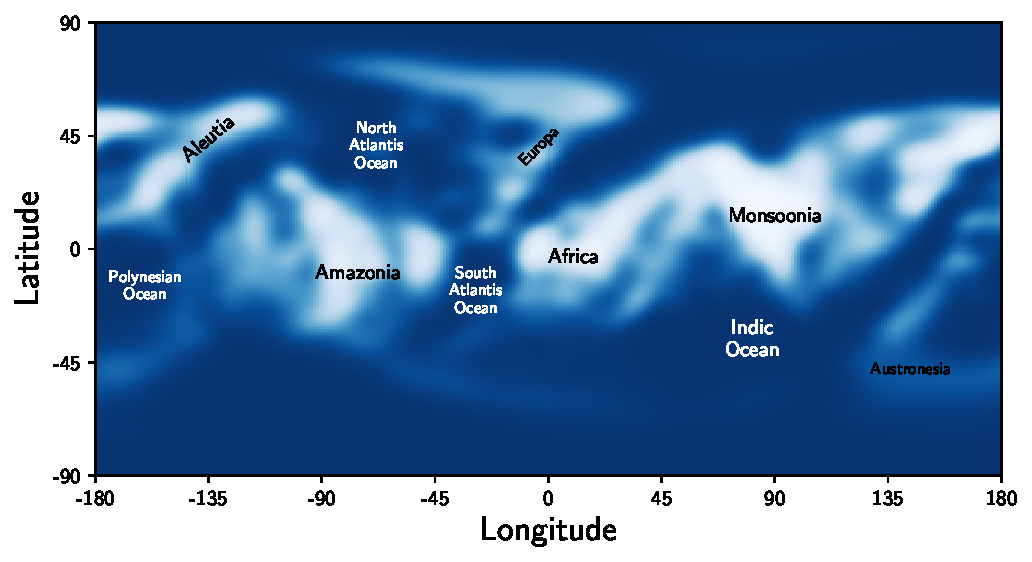
\includegraphics[width=\linewidth]{figures/map_labels.pdf}
    \caption{\label{fig:map_labels}
             Map of Sol d with the major features indicated with suggested
             names.
             \codelink{earthshine_S1_S2}
             }
    \end{centering}
\end{figure}

\todo{(comparison of inferred features to ``model'' (Earth))}

\todo{No zonal cloud bands: prior.}

\section{Conclusion}
\label{sec:conclusion}

\todo{(summarize)}

\todo{(utility for \TESS background removal)}

\todo{(talk abt prospects for doing this analysis with exoplanets)}


\acknowledgements{\todo{(Artist acknowledgement)} The authors gratefully 
acknowledge Dan Foreman-Mackey, David W Hogg, Ben Pope, \todo{and ...} 
for useful conversations. Crucial parts of this work were carried out at the 
TESS Data Workshop, hosted by Space Telescope Science Institute, and the 
Building Early Science with TESS Workshop, hosted by the University of Chicago.}
\facility{TESS}
\software{Astropy, Matplotlib, Numpy, \starry \citep{Luger2019}, 
TensorFlow \citep{Abadi2015}, \spiceypy \citep{Annex2019}}
% Bibliography
\pagebreak
\bibliography{bib}

\end{document}
